\documentclass[11pt]{article}

\usepackage[letterpaper, margin=1in]{geometry}

\usepackage[spanish]{babel}
\usepackage[utf8]{inputenc}
\usepackage{multirow}
\usepackage{tabularx}
\usepackage{longtable}

\usepackage{listings}% Escribir código de programación



%Figuras
\usepackage{graphicx, subfigure}
\usepackage[]{tikz}
\usepackage{pbox}

%Matemática
\usepackage{amsmath}
\usepackage{amssymb}

%Símbolos mate extra (alfabetos, etc.)
\usepackage{mathrsfs}


%Algoritmos
\usepackage{float}
\usepackage{algorithm}
\usepackage{algorithmicx}
\usepackage{algpseudocode}
\usepackage{listings}


\usepackage{color}
\usepackage{hyperref}

\usepackage{mdframed}
\usepackage{tcolorbox}
\usepackage{multicol}
\usepackage{booktabs}
\usepackage{tabulary}
\definecolor{darkblue}{rgb}{0 , 0.054 , 0.196}



\title{Reporte de laboratorio 6}
\author{Laura Rincón Riveros - B55863\\Esteban Vargas Vargas - B16998\\ Grupo 3}

\begin{document}

\maketitle
\hrule
\hrule
\tableofcontents
\hspace{5mm}
\hrule
\hrule

%%%%%%%%%%%%%%%%%%%%%%%%%%%%%%%%%%%%
\section{Introducción}
%%%%%%%%%%%%%%%%%%%%%%%%%%%%%%%%%%%%

En el presente laboratorio se desarrolló una estructura de datos llamada grafo; como se muestra a continuación:


\newpage
%%%%%%%%%%%%%%%%%%%%%%%%%%%%%%%%%%%%
\section{Desarrollo}
%%%%%%%%%%%%%%%%%%%%%%%%%%%%%%%%%%%%

%%%%%%%%%%%%%%%%%%%%%%
\subsection{Clase Vertex}
%%%%%%%%%%%%%%%%%%%%%%

Se creó una clase Vertex, la cuál representa los vértice del grafo, en ella se encuentra el valor del dato, su nivel y un atributo booleano para comprobar si fue visitado(en el caso de la impresión). A continuación se presenta el archivo Vertex.h: 

\subsubsection{Vertex.h}
\lstset {language=C}
\begin{lstlisting}

#ifndef VERTEX_H
#define VERTEX_H

class Vertex {
public:

    char* value;
    bool visited;
    int nivel;

    Vertex();

    Vertex(bool visit, char* val);

    //virtual ~Vertex();

private:

};

#endif /* VERTEX_H */




\end{lstlisting}
\newpage
%%%%%%%%%%%%%%%%%%%%%%
\subsubsection{Clase Matrix}
%%%%%%%%%%%%%%%%%%%%%%

La clase Matrix, implementa una puntero doble para organizar los datos según sus enlaces, a lo que se conoce como matriz de adyacencia. 

Posee el atributo que es el contenido y su tamaño, como es una matriz cuadrada solo es necesario un valor. 

Esta es capaz de ampliar o reducir su tamaño, con las funciones changesize, removerowcolumn; y de encontrar un valor en específico con findedge.

\lstset {language=C}
\begin{lstlisting}

#include <iostream>
#include <string.h>
using namespace std;

class Matrix {
public:

    Matrix(int tam);

    Matrix(int** values, int tam);

    virtual ~Matrix();
    
        
    int** matrix;
    int size;

    
    void change_size(int new_size);
    
    void remove_rowcolumn(int row);
    
    int* find_edge(int e);
    
    void print();

};

#endif /* MATRIX_H */


\end{lstlisting}



%%%%%%%%%%%%%%%%%%%%%%
\subsubsection{Clase Grafo}
%%%%%%%%%%%%%%%%%%%%%%
La clase Grafo, donde se implementan propiamente esta estructura de datos, utiliza las clases anteriormente mencionadas. El grafo es capaz de agregar vértices y aristas, eliminarlos y de imprimir su contenido de diversas maneras (sin orden definido y usando dos distintos algoritmos de búsqueda). 
\newpage 
\subsubsection{Grafo.h}
\lstset {language=C}
\begin{lstlisting}
#ifndef GRAFO_H
#define GRAFO_H

#include "Vertex.h"
#include "ListaConArreglo.h"
#include "Matrix.h"

class Grafo {
public:

    int hight;
    int depth;
    Vertex* source;
    int num_vertex;
    ListaConArreglo<Vertex>* vertices;
    Matrix* adjacency;
    
    int name;

    Grafo();

    virtual ~Grafo();
    
    void add_vertex(char* v);
    
    void remove_Vertex(Vertex v);
    
    void add_Edge(Vertex v1, Vertex v2);
    
    void removeEdge(int e);
    
    void display();
    
    void bsf();
    
    void search_bfs(int row, int column);
    
    void dfs();
    
    void search_dfs(int row, int column);

private:

};


#endif /* GRAFO_H */


\end{lstlisting}

En la figura se presenta el diagrama UML de grafo:
\begin{figure}[h!]
\centering
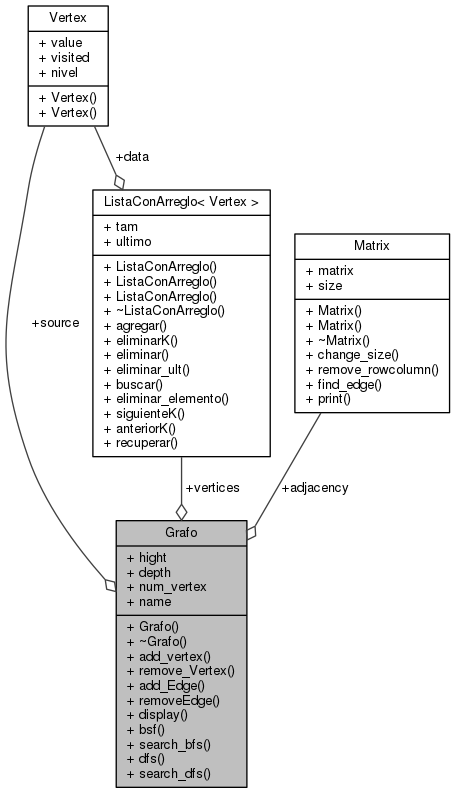
\includegraphics[width=0.7\textwidth]{imagencita.png}
\caption{\label{fig:umlcalc} Diagrama colaboración clase Grafo}
\end{figure}


%%%%%%%%%%%%%%%%%%%%%%
\subsection{Main}
En el main se creó un objeto grafo. Para ello fue necesario agregarle los vértices deseados y las aristas. A continuación se presenta el código:


\lstset {language=C}
\begin{lstlisting}
#include <cstdlib>

#include "Grafo.h"

#include <string.h>
#include <iostream>
using namespace std;


int main(int argc, char** argv) {
   
    
 Grafo* prueba= new Grafo();
  char* ax = new char('A');
  prueba->add_vertex(ax);

  char* bx = new char('B');
  prueba->add_vertex(bx);
  //prueba->adjacency->print();//***impresion

  char* cx = new char('C');
  prueba->add_vertex(cx);
  //prueba->adjacency->print();//***impresion

  char* dx = new char('D');
  prueba->add_vertex(dx);
  cout<<"Matriz 4x4 creada para un grafo de 4 vertices"<<endl;
  prueba->adjacency->print();//***impresion

  Vertex a;
  a.value=ax;

  Vertex b;
  b.value= bx;

  Vertex c;
  c.value= cx;
  
  Vertex d;
  d.value= dx;  

  prueba->add_Edge(a,b);
  prueba->add_Edge(b,d);  
  prueba->add_Edge(c,d);
  prueba->add_Edge(c,a);
  
  cout<<"Matriz de adyacencia"<<endl;  
  prueba->adjacency->print();
  
  cout<<"Display del grafo"<<endl;
  prueba->display();
  cout<<"Depth first search"<<endl;  
  prueba->dfs();
  cout<<"Breadth first search"<<endl;  
  prueba->bsf();


  /*prueba->removeEdge(1);
  prueba->adjacency->print();*/
    
    
  return 0;
}
\end{lstlisting}
%%%%%%%%%%%%%%%%%%%%%%
Finalmente se muestra la salida del programa con una captura de pantalla:

\begin{figure}[h!]
\centering
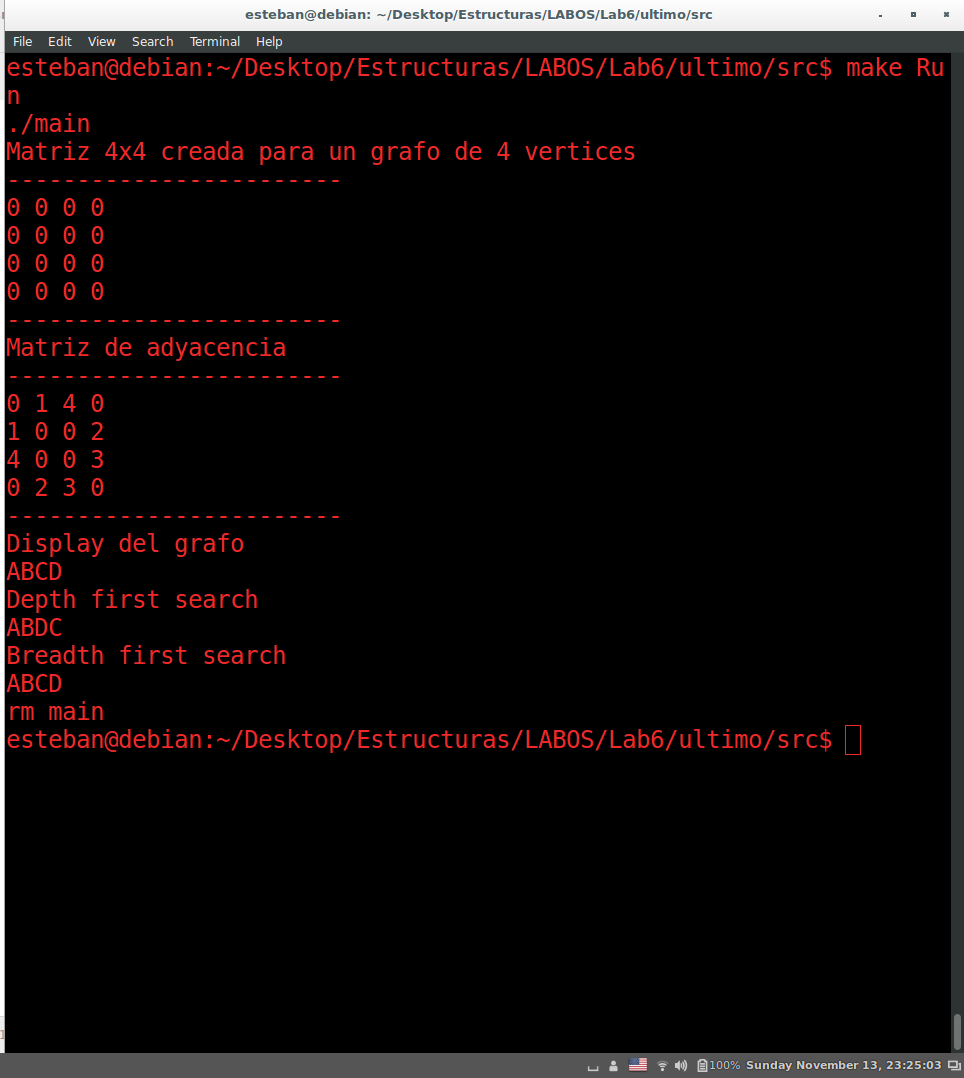
\includegraphics[width=0.9\textwidth]{cap.png}
\caption{\label{fig:2} Salida programa}
\end{figure}





\newpage
%%%%%%%%%%%%%%%%%%%%%%%%%%%%%%%%
\section{Conclusiones}
%%%%%%%%%%%%%%%%%%%%%%%%%%%%%%%%
\begin{itemize}
\item Se logró implementar un grafo mediante una matriz de adyacencia.
\item Se realizó búsqueda en el grafo mediante \textit{''Depth first search''}.
\item Se realizó búsqueda en el grafo mediante \textit{''Breadth first search''}.
\end{itemize}
\newpage
 
\section{Anexos}
\subsection{Vertex.cpp}
\lstset {language=C}
\begin{lstlisting}
#include "Vertex.h"

Vertex::Vertex() {
    value = 0x0;
    visited = false;
    nivel=0;
}

Vertex::Vertex(bool visit, char* val) {

    value =  val;
    visited = visit;
    nivel=0;

}

//Vertex::~Vertex() {
//    delete value;
//};

\end{lstlisting}
\newpage 
\subsection{Matrix.cpp}
\lstset {language=C}
\begin{lstlisting}
#include "Matrix.h"

#include <string.h>
#include <iostream>
using namespace std;

Matrix::Matrix(int tam){
    matrix = new int*[tam];
    size = tam;

    
    for (int i = 0; i < size; i++) {
        matrix[i] = new int[size];
        }
    
    for(int row=0;row<size;row++){
        for (int column=0;column<size;column++){
            matrix[row][column]= 0;

        }
    }
    
}

Matrix::Matrix(int** values, int tam) {

    matrix = values;
    size= tam;

}

Matrix::~Matrix() {
    delete matrix;
}

void Matrix::change_size(int new_size){

    int** temp= new int*[new_size];
      for (int i = 0; i < new_size; i++) {
        temp[i] = new int[new_size];
        }
    

    for(int row=0;row<new_size;row++){
        for (int column=0;column<new_size;column++){
            if(row<size && column<size){
                temp[row][column]=matrix[row][column];
            }
            else{
                temp[row][column]= 0;
            }
        }
    }

    matrix = temp;
    size = new_size;
}

void Matrix::remove_rowcolumn(int rc){
    int** temp= new int*[this->size-1];
    
    for (int i = 0; i < this->size-1; i++) {
      temp[i] = new int[this->size-1];
    }
    
    int hor;
    int ver;
    
     for(int row=0;row<(this->size-1);row++){
        for (int column=0;column<this->size-1;column++){
            hor=row;
            ver=column;
            
            if(row>=(rc-1)){
                hor++;
            }
            if(column>=(rc-1)){
                ver++;
            }
            temp[row][column]=matrix[hor][ver];           
        }
    }
    
    matrix=temp;
    size= size-1;
    
}

int* Matrix::find_edge(int e){

    for(int row=0;row<size;row++){
        for (int column=0;column<size;column++){
            if(matrix[row][column]== e){
                return &(matrix[row][column]);
            }
        }
    }
    return 0x0;
}

void Matrix::print(){
    cout<<"------------------------"<<endl;
     for(int i = 0; i < size; i++){
        for(int j=0; j< size ;j++){
            cout << matrix[i][j] << " ";
        }
        cout << endl;
    }
    cout<<"------------------------"<<endl;
}
\end{lstlisting}
\newpage 
\subsection{Grafo.cpp}
\lstset {language=C}
\begin{lstlisting}
#include "Grafo.h"
#include <stack>


Grafo::Grafo() {
    hight=0;
    depth=0;
    num_vertex=0;
    source=0x0;
    vertices= new  ListaConArreglo<Vertex>();
    adjacency = new Matrix(0);

    name=0;
};


Grafo::~Grafo() {
    delete vertices;
    delete adjacency;
}

void Grafo::add_vertex(char* v){
    Vertex* n = new Vertex(false, v);
    if(num_vertex==0){
        source = n;
    }

    vertices->agregar(*n); //agrega en la lista de vertices
    adjacency->change_size(adjacency->size+1);
    num_vertex++;

}

void Grafo::remove_Vertex(Vertex v){
    int index;
   
    for(int i=0; i<vertices->tam; i++){
            if(*(vertices->data[i].value)==*(v.value)){
                index=i;
            }
        }
    vertices->eliminarK(index);

    adjacency->remove_rowcolumn(index+1);
    num_vertex--;
}

void Grafo::add_Edge(Vertex v1, Vertex v2){
    if(vertices->tam>0){

        int v_1;
        int v_2;
        
        
        
        for(int i=0; i<vertices->tam; i++){
            if(*(vertices->data[i].value)==*(v1.value)){
                v_1=i;
            }
            if(*(vertices->data[i].value)==*(v2.value)){
                v_2=i;
            }
        }

        v2.nivel= v1.nivel+1;

        name=name+1;
        adjacency->matrix[v_1][v_2]=name;
        adjacency->matrix[v_2][v_1]=name;

    }
}

void Grafo::removeEdge(int e){
   
    *(adjacency->find_edge(e))=0;
    *(adjacency->find_edge(e))=0;  
}

void Grafo::display(){
    
  for(int i=0;i<this->num_vertex;i++){
    cout<<*(this->vertices->recuperar(i).value);
  }
  cout<<endl;
}

void Grafo::bsf(){  
    cout<<*(source->value);
    vertices->data[0].visited=true;
    search_bfs(0,0);
    
    cout<<""<<endl;
    for(int i=0; i<num_vertex; i++){
        vertices->data[i].visited=false;
    }
}

void Grafo::search_bfs(int row, int column){ 
    
    ListaConArreglo<int> stack;
    
    if(adjacency->matrix[row][column]>0 && vertices->data[row].visited==false){
        
        cout<< *(vertices->data[row].value);
        vertices->data[row].visited=true;
        stack.agregar(row);

    }
    
    if(row<num_vertex-1){
        search_bfs(row+1,column);
    }
    if(stack.tam>0){
        search_bfs(0,stack.data[0]);
        stack.eliminar();
    }
    
}

void Grafo::dfs(){
    cout<<*(source->value);
    vertices->data[0].visited=true;
    search_dfs(0,0);
    
    cout<<""<<endl;
    
    for(int i=0; i<num_vertex; i++){
        vertices->data[i].visited=false;
    }
}


void Grafo::search_dfs(int row, int column){ 
    if(adjacency->matrix[row][column]>0 && vertices->data[row].visited==false){ 
        cout<< *(vertices->data[row].value);
        vertices->data[row].visited=true;
        search_dfs(0,row);
    }
    else{
        if(row<num_vertex-1){
            search_dfs(row+1, column);
        }
    }
    
}




\end{lstlisting}


\end{document}
